\documentclass[10pt,a4paper]{article}
\usepackage[utf8]{inputenc}
\usepackage{amsmath}
\usepackage{gensymb}
\usepackage{amsfonts}
\usepackage{siunitx}
\usepackage[european]{circuitikz}
\usepackage{geometry}
\newgeometry{tmargin=2cm, bmargin=2cm, lmargin=2cm, rmargin=2cm}
\usepackage{amssymb}
\usepackage{polski}
\usepackage{graphicx}
\author{\textbf{T. Fąs}}
\title{\textbf{WAHADŁA SPRZĘŻONE}}
\begin{document}
\maketitle

\begin{center}
\textbf{\subsection*{STRESZCZENIE}}
\end{center}
W doświadczeniu wyznaczano współczynnik sprężystości $k$ sprężyny dwoma metodami. Otrzymano ostateczną wartość $k=(26,295030\pm0,000036)$ N/m.


\begin{center}
\textbf{\subsection*{WSTĘP}}
\end{center}
Ruch dwóch identycznych wahadeł o momencie bezwładności $I$ połączonych sprężyną o współczynniku sprężystości $k$ silnie zależy od warunków początkowych. Ich okresy różnią się zależności od wzajemnego położenia początkowego.

\begin{figure}[h!]
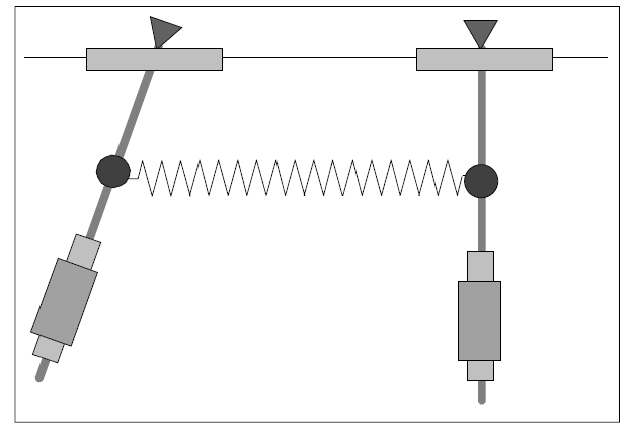
\includegraphics[width=10cm]{rap12ukl} 
\centering
\caption{Wahadła sprzężone.}
\end{figure}

 Dla układu przedstawionego na Rysunku 1, możliwe są następujące warunki:
 \begin{enumerate}
 \item Jeżeli wahadła są wychylone o taki sam kąt w tym samym kierunku, to ich okresy są identyczne i dane wzorem:
 \begin{equation}
 T_{1}=2\pi\sqrt{\dfrac{I}{mgr}}.
 \end{equation}
 \item Jeżeli są wychylone o taki sam kąt, ale w przeciwne strony, to okres ich ruchu dany jest wzorem:
 \begin{equation}
  T_{2}=2\pi\sqrt{\dfrac{I}{mgr+2ka^2}}.
 \end{equation}
 \item Jeżeli jedno z wahadeł jest unieruchomione, to okres drgań drugiego z nich wyraża się wzorem:
 \begin{equation}
  T_{0}=2\pi\sqrt{\dfrac{I}{mgr+ka^2}}.
 \end{equation}
 \item Jeżeli jedno z wahadeł początkowo spoczywa, to dochodzi do zjawiska okresowej zmiany amplitudy drgań wahadeł, czyli dudnień. W takim wypadku okres szybkich drgań dany jest wzorem:
 \begin{equation}
 T_{s}=\dfrac{2T_{1}T_{2}}{T_{1}+T_{2}},
 \end{equation}
 a okres dudnień dany jest wzorem:
 \begin{equation}
 T_{d}=\dfrac{2T_{1}T_{2}}{T_{1}-T_{2}}.
 \end{equation}
 \end{enumerate}
Przy czym w wzorach $m$ oznacza masę wahadła, $a$ jest odległością sprężyny od osi obrotu, a $r$ odległością środka masy od osi obrotu.

Doświadczenie miało na celu pomiar tych wszystkich okresów drgań, sprawdzenie, czy zmierzone wartości $T_{s}$ i $T_{d}$ są zgodne z ich wartościami teoretycznymi oraz wyznaczenie współczynnika sprężystości $k$. 

Inną metodą wyznaczania współczynnika sprężystości jest wykorzystanie prawa Hooke'a, które głosi, iż wydłużenie $\Delta x$ sprężyny jest wprost proporcjonalne do działającej na nią siły $F$. Czyli:
\begin{equation}
F=k\Delta x.
\end{equation}
 Mierząc zmianę wydłużenia sprężyny przy działaniu znanej siły można w prosty sposób wyznaczyć stałą sprężystości $k$.




\begin{center}
\textbf{\subsection*{UKŁAD DOŚWIADCZALNY}}
\end{center}
Układ doświadczalny składał się z dwóch wahadeł, sprężyny, nitki, zapalniczki, stopera, miarki, ciężarków, ostrza pryzmatycznego i wagi. 

Przy pomocy stopera mierzono okresy wahadeł, a przy pomocy nitki wiązano wahadła, by zwalniać je w tej samej chwili przepalając sznurek. Do przytrzymania jednego z wahadeł wykorzystano statyw.

 W trakcie wykonywania pomiarów związanych z prawem Hooke'a sprężyna była zawieszona na statywie. Na sprężynie zawieszano kolejne ciężarki, a odchylenie mierzono przy pomocy miarki. 
 
 Również przy pomocy miarki zmierzono odległość sprężyny od osi obrotu. Przy pomocy ostrza pryzmatycznego wyznaczono położenie środka masy i miarką wyznaczono jego odległość od osi obrotu.

Aby upewnić się, czy wahadła są identyczne, badano ich synchronizację w trakcie kilkuminutowego ruchu. Stwierdzono, że ruch wahadeł jest zgodny w odpowiednio długim okresie.

\begin{center}
\textbf{\subsection*{WYNIKI POMIARÓW}}
\end{center}

W trakcie pomiarów mierzono, dla lepszej dokładności, dziesięć okresów $T_{1}$, $T_{2}$ i $T_{0}$ oraz pięć okresów $T_{s}$. Planowano również zmierzyć wielokrotność okresów $T_{d}$, jednakże uciekający czas eksperymentu na to nie pozwolił. Wyniki pomiarów przedstawiono w Tabeli 1.
\begin{table}[h!]
\centering
\caption{Wyniki pomiarów okresów.}
\begin{tabular}{|c|c|c|c|c|}
\hline
$10T_{1}$ [s]& $10T_{2}$ [s]& $T_{d}$ [s]& $5T_{s}$ [s]& $10T_{0}$ [s]\\ \hline
18,91     & 16,06     & 20,75   & 9,44     & 17,18     \\ \hline
18,88     & 15,78     & 20,50   & 9,41     & 17,18     \\ \hline
18,88     & 16,08     & 20,87   & 9,41     & 17,19     \\ \hline
18,81     & 16,00     & 20,91   & 9,43     & 17,16     \\ \hline
18,97     & 15,84     & 20,97   & 9,50     & 17,19     \\ \hline
19,03     & 16,00     & 20,82   & 9,53     & 17,13     \\ \hline
18,87     & 15,94     & 20,31   & 9,50     & 17,10     \\ \hline
18,84     & 15,93     & 20,87   & 9,47     & 17,15     \\ \hline
18,78     & 16,00     & 20,78   & 9,47     & 17,13     \\ \hline
18,90     & 15,97     & 20,69   & 9,41     & 17,19     \\ \hline
\end{tabular}
\end{table}
Pomiary przeprowadzono dla wartości $r=81,9$ cm, $a=41,5$ cm, masa m wahadła wynosiła $m=(3000\pm40)$ g. Rozdzielczość stopera wynosiła $\Delta_{t}=0,01$ s, a czas reakcji obserwatora wynosił $t_{r}=0,3$ s.

W przypadku rozciągania sprężyny wykonano pomiar długości od górnej krawędzi statywu do końca sprężyny. Rożnica pomiędzy długością przy obciążeniu, a długością bez obciążenia jest szukanym wydłużeniem sprężyny. Pomiar masy był dokonywany przy pomocy wagi i ponawiany po każdym dodaniu nowego ciężarka. Tabela 2 przedstawia wyniki pomiarów dla tej części eksperymentu.


\begin{table}[h!]
\centering
\caption{Wyniki pomiarów: prawo Hooke'a.}
\begin{tabular}{|c|c|c|c|c|c|c|c|c|c|c|c|}
\hline
Masa $m$ ciężarków [g] & 0  & 120,49 & 140,30 & 159,79 & 179,38 & 199,20 & 219,08 & 239,79 & 278,81 & 308,33 & 378,75 \\ \hline
Długość x [cm]         & 34,0 & 38,3   & 39,5  & 40,0     & 40,7   & 41,5  & 42,3   & 43,0 & 44,2   & 45,7   & 47,9   \\ \hline
\end{tabular}
\end{table}

\begin{center}
\textbf{\subsection*{ANALIZA DANYCH}}
\end{center}
Pomiary czasu dla każdej serii postanowiono uśrednić, korzystając ze średniej arytmetycznej:
\begin{equation}
\bar{T}=\sum_{i=1}^{N}\dfrac{T_i}{N},
\end{equation}
gdzie $N$ jest liczbą pomiarów, w tym przypadku $N=10$. 

Ostateczne niepewności pomiarów czasu $u_{T}$ obliczono, korzystając z odchylenia standardowego średniej $s$, które jest wyrażone wzorem:
\begin{equation}
s^2_{T}=\sum_{i=1}^{N}\dfrac{(T_{i}-\bar{T})^2}{N(N-1)} \quad \cite{tay2}
\end{equation}
oraz ze związku pomiędzy odchyleniem standardowym średniej, a maksymalnym dopuszczalnym błędem pomiaru $\Delta$:
\begin{equation}
u_{T}=\sqrt{s^2_{t}+\dfrac{\Delta_{T}^2}{3}+t_{r}^2}.
\end{equation}

Następnie przeniesiono to na grunt pojedynczych okresów, czyli wielkości podzielono przez 10 lub 5. Wyniki analizy przedstawia Tabela 3.

\begin{table}[h!]
\centering
\caption{Analiza okresów.}
\begin{tabular}{|c|c|c|c|c|c|}
\hline
                      & $10T_{1}$ [s] & $10T_{2}$ [s] & $T_{d}$ [s] & $5T_{s}$ [s] & $10T_{0}$ [s] \\ \hline
Średnia               & 18,89         & 15,96         & 20,75       & 9,46         & 17,16         \\ \hline
Odchylenie            & 0,023         & 0,029         & 0,064       & 0,014        & 0,010         \\ \hline
Pojedynczy okres      & 1,889         & 1,596         & 20,75      & 1,891        & 1,716         \\ \hline
Ostateczna niepewność & 0,030         & 0,030         & 0,31       & 0,060        & 0,030         \\ \hline
\end{tabular}
\end{table}

Porównanie okresów $T_{s}$ i $T_{d}$ z ich wartościami teoretycznymi wynikającymi z Równania (4) i Równania (5) przeprowadzono, korzystając z testu $3\sigma$. Polega on na sprawdzeniu, czy różnica dwóch porównywanych wielkości jest mniejsza od trzykrotności niepewności tej różnicy. W tym przypadku niepewność związaną z wartościami teoretycznymi $T_{s}$ i $T_{d}$ obliczono, korzystając z metody propagacji małych błędów. Wzór przenoszenia niepewności w tej metodzie jest następujący:

 \begin{equation}
 u_{f}^2=\sum_{i=1}^n \left( \dfrac{\partial f}{\partial x_{i}}u_{i}\right)^2,
 \end{equation}
 gdzie wielkość $f$ zależy od wielkości $x_{i}$ o niepewnościach $u_{i}$ \cite{tay1}. 
 
 Otrzymano wartości $T_{s2}=1,730\pm0,022$ s oraz $T_{d2}=20,60\pm3,08$ s. Tak więc różnica $T_{s}-T_{s2}$ wynosi 0,161 s przy niepewności 0,064 s, a różnica $T_{d}-T_{d2}$  
 wynosi 0,15 s przy niepewności 3,1 s. Jak widać, obie te wielkości są ze sobą zgodne na poziomie $3\sigma$. 
 
W dalszej części analizy skupiono się na współczynniku sprężystości $k$. Korzystając z Równania (1), Równania (2) i Równania (3) oraz wiedząc że $2\pi=T_{i}\omega_{i}$ otrzymano:
\begin{equation}
k_{1}=\dfrac{\left(\omega_{2}^2-\omega_{1}^2\right)mgr}{2a^2\omega_{1}^2}.
\end{equation}
\begin{equation}
k_{2}=\dfrac{\left(\omega_{0}^2-\omega_{1}^2\right)mgr}{a^2\omega_{1}^2}.
\end{equation}
Niepewność tych współczynników obliczono, korzystając z Równania (10), uprzednio wyznaczając niepewności $\omega_{i}$. Za niepewności pomiaru $r$ i $a$ przyjęto 1 mm, ponieważ ustawienie miarki dokładnie w punkcie obrotu było utrudnione. Wykorzystano wartość $g=9,80665$ m/s$^2$. Otrzymano wartości: $k_{1}=(28,0\pm4,6)$ N/m, $k_{2}=(29,6\pm8,0)$ N/m. Przy tak dużych niepewnościach wartości bez problemu przechodzą test $\sigma$. Aby uzyskać lepszą ocenę wartości współczynnika $k$ obliczono średnią ważoną obu otrzymanych współczynników. 
Średnia ważona $N$ wielkości $x_{i}$ o niepewnościach $u_{i}$ zdefiniowana jest w następujący sposób:
 	\begin{equation}
 	\bar{x}_{w}=\dfrac{\sum_{i=1}^{N}\dfrac{x_i}{u_{i}^2}}{\sum_{i=1}^{N}\dfrac{1}{u_{i}^{2}}}.
 	\end{equation}
 Niepewności średniej ważonej wrażają się w następującymi wzorami:
 \begin{eqnarray}
 u^{2}_{int}=\dfrac{1}{\sum_{i=1}^{N}\dfrac{1}{u_{i}^2}}, \\
 u^{2}_{ext}=\dfrac{u_{int}^2}{N-1}\sum_{i=1}^{N}\left(\dfrac{x_{i}-\bar{x}_{w}}{u_{i}}\right)^2.
 \end{eqnarray}
 Jako ostateczną niepewność niepewność wielkości $\bar{x}_{w}$ wybiera się większą z niepewności $u_{int}$ lub $u_{ext}$ \cite{tay4}.
 
Po podstawieniu odpowiednich wartości otrzymano $k=28,4\pm4,2$ N/m.

W przypadku analizy danych związanych z prawem Hooke'a niepewność pomiaru masy wynosiła 0,01 g, a niepewność długości przyjęto jako 3 mm, ponieważ ciężko było znaleźć łatwo dostępny punkt charakterystyczny znakujący koniec sprężyny. Aby wyznaczyć współczynnik sprężystości postanowiono do otrzymanych danych dopasować prostą. Jako, że niepewność związana z wydłużeniem sprężyny jest procentowo większa od niepewności pomiaru masy ciężarków, to na osi OY zdecydowano się odłożyć wielkość $\Delta x$. Dodatkowo, dla wygody analizy, zamieniono jednostki na metry i kilogramy i obliczono siłę ciężaru związaną z danym ciężarkiem. Niepewność wydłużenia obliczono z Równania (10). Ostateczne wartości punktów wraz z niepewnościami przedstawiono w Tabeli 4.
 
 \begin{table}[h!]
\centering
\caption{Analiza danych: prawo Hooke'a.}
\begin{tabular}{|c|c|c|c|c|c|c|c|c|c|c|c|}
\hline
Ciężar mg [N]             & 0 & 1,182 & 1,376 & 1,567 & 1,759 & 1,953 & 2,148 & 2,352 & 2,734 & 3,024 & 3,714 \\ \hline
Wydłużenie $\Delta x$ [m] & 0 & 0,043 & 0,055 & 0,060 & 0,067 & 0,075 & 0,083 & 0,090 & 0,102 & 0,117 & 0,139 \\ \hline
Niepewność wydłużenia [m]    & 0 & 0,004 & 0,004 & 0,004 & 0,004 & 0,004 & 0,004 & 0,004 & 0,004 & 0,004 & 0,004 \\ \hline
\end{tabular}
\end{table}
 
Z Równania (6) wynika, że efektem dopasowania powinna być prosta, o współczynniku kierunkowym równym odwrotności stałej sprężystości: $\Delta x=mg/k$. Aby dopasować prostą do punktów z Tabeli 4 posłużono się programem SciDAvis. Otrzymaną w ten sposób krzywą najlepszego dopasowania przedstawiono na Rysunku 2.


 \begin{figure}[h!]
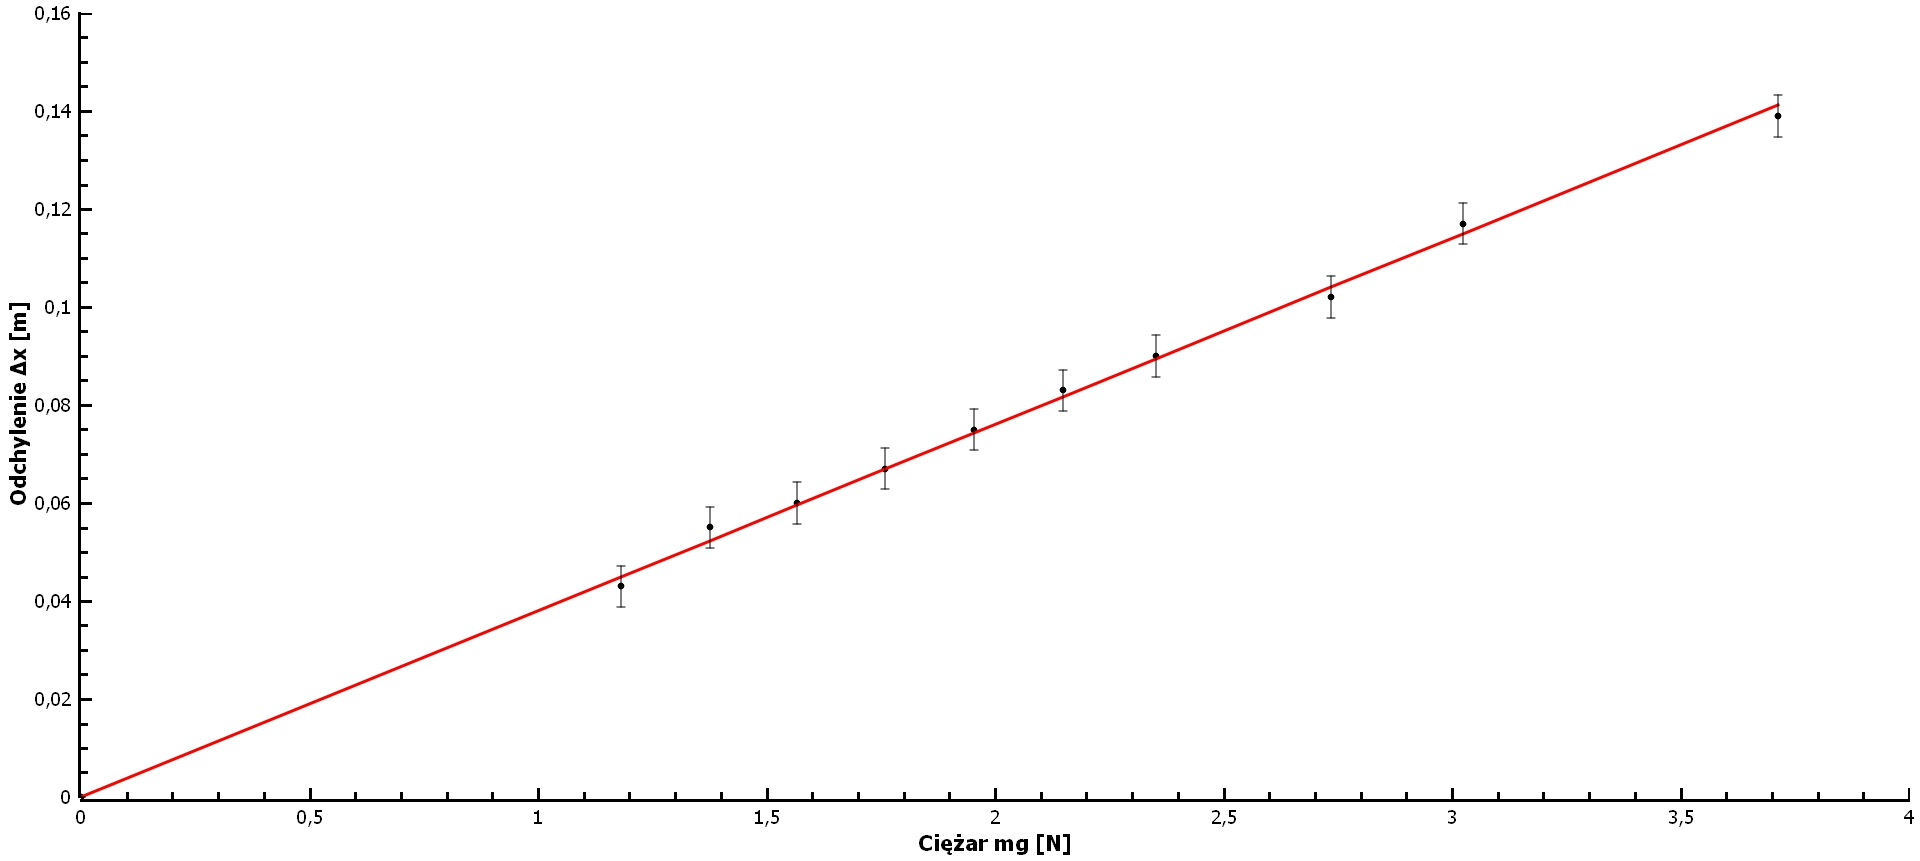
\includegraphics[width=15cm]{rap12rys1} 
\centering
\caption{Wahadła sprzężone.}
\end{figure}
 
Współczynnik kierunkowy tej krzywej wynosi $1/k=0,038030000000\pm0,000000052727$ m/N, a wartość $\chi^2=1,48$. Wartość ta jest mniejsza od wartości krytycznej, tak więc dane są niesprzeczne z Równaniem (6). 

Odwracając współczynnik kierunkowy otrzymano wartość współczynnika $k=26,295030\pm0,000036$ N/m. Wielkość ta, na mocy testu $3\sigma$ jest zgodna z poprzednio otrzymaną wartością współczynnika. Zastosowanie średniej ważonej do obu tych wielkości zwraca praktycznie taki sam wynik, jak obliczony właśnie współczynnik.
Dlatego też ostateczna wartość stałej sprężystości wynosi $k=26,295030\pm0,000036$ N/m.
\begin{center}
\textbf{\subsection*{DYSKUSJA WYNIKÓW I WNIOSKI}}
\end{center} 
Otrzymana wartość współczynnika cechuje się niewiarygodnie niską niepewnością, jednakże patrząc na bardzo dobre dopasowanie prostej do punktów oraz na wartości niepewności, które same w sobie są niskie, to otrzymanie takiej wartości dziwi trochę mniej. Zdecydowanie mniej dziwi zgodność wyników w przypadku okresów dudnień i drgań szybkich. Dysponując wielokrotnymi pomiarami oraz zsynchronizowanymi wahadłami otrzymanie zgodnych wyników było niemal pewne. Ostatecznie można uznać uzyskane wynika za zadowalające. 


\begin{center}
\begin{thebibliography}{9}


 \bibitem{tay2}
 J. R. Taylor,
 \emph{Wstęp do analizy błędu pomiarowego},
 PWN, Warszawa, 1995, s. 101.
 
 
\bibitem{tay1}
 J. R. Taylor,
 \emph{Wstęp do analizy błędu pomiarowego},
 PWN, Warszawa, 1995, s. 175.
 
  \bibitem{tay4}
 J. R. Taylor,
 \emph{Wstęp do analizy błędu pomiarowego},
 PWN, Warszawa, 1995, s. 169. 


 \end{thebibliography}

\end{center}


\end{document}